\documentclass[12pt, letterpaper]{report}
\usepackage{graphicx}
\usepackage{hyperref}
\usepackage{amssymb}
\usepackage{amsmath}
\usepackage{float}
\usepackage{mathtools}
\usepackage{enumitem}
\usepackage[margin=1in]{geometry}
\usepackage[figurename=Figura]{caption}
\title{Actividad: Separación de minerales}
\author{Juan Pablo Guerrero Escudero, A01706810}
\date{17 abril, 2024}
\begin{document}
\maketitle
\subsection*{Introducción}
En éste reporte, se analizará el fenómeno que sucede cuando una mezcla de minerales de fosfato y cuarzo 
se libera hacia una cámara, donde un campo eléctrico induce la separación de las partículas. Éstas partículas, al tener 
diferentes propiedades dieléctricas, seguirán trayectorias distintas. En el análisis, se hace uso de varios conceptos relacionados al 
electro-magnetismo, tales como la Ley de Coulomb y el Campo Eléctrico. Además, para el cálculo de la posición, velocidad y aceleración 
se utilizan las leyes de Newton, así como conceptos de cálculo integral y diferencial para el cálculo de las ecuaciones 
representativas de posición, velocidad y aceleración. 

\subsection*{Desarrollo teórico}
\begin{figure}[H]
    \centering
    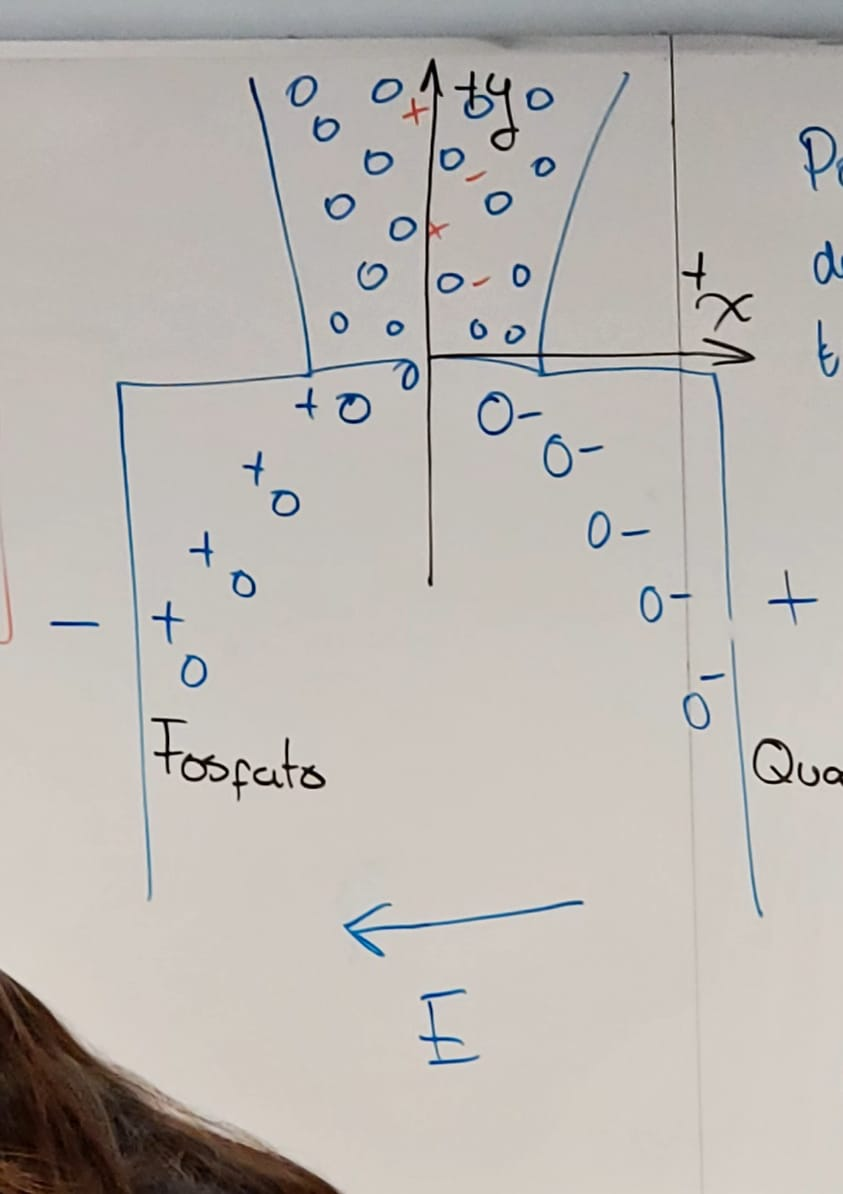
\includegraphics[height = 8cm]{2024-04-17_DiagramaSeparacionMinerales.jpeg}
    \caption{Diagrama de separación de minerales}
    \label{fig:fig1}
\end{figure}
En la figura \ref{fig:fig1}, tenemos una situación en donde las partículas son ingresadas en una cámara que contiene un campo eléctrico, que está en dirección de la parte 
negativamente cargada de éste. En la cámara, existe un campo eléctrico, el cuál se define como $\vec{E} = \vec{F}/Q_1$, que corresponde con la fórmula 
para el cálculo convencional de éste. Además, gracias a Coulomb, otra manera de definir el campo eléctrico es $\vec{E} = k(\frac{Q_1}{R^3})\vec{R}$, medido en volts por metro. 
Además, tenemos las siguientes restricciones iniciales: 
\begin{enumerate}
\item Las partículas parten del origen (0, 0), de acuerdo a los ejes coordenados en el diagrama. 
\item La velocidad inicial $V_0 = 0$. 
\item El movimiento es en $\mathbb{R}^2$. 
\end{enumerate}
Con ésto, el objetivo es obtener las fórmulas que nos digan la posición $x(t)$ y $y(t)$, La velocidad $V_x(t)$ y $V_y(t)$, 
y la aceleración $a_x(t)$, $a_y(t)$. \\

Para ésto, es conveniente hacer el análisis individual en cada eje, para obtener las fórmulas necesarias. 
\subsubsection*{Análisis en Eje X}
En primer lugar, la fuerza en x resulta $F_x = (-q)(-E)$, pero al hacer el producto resulta $F_x = qE$, siendo $q$ la carga y $E$ el campo eléctrico. Aquí, podemos usar la fórmula de Newton $F = ma$ para 
introducir el tiempo por medio de $a_x(t)$, lo cuál al sustituir en la fórmula de $F_x$, resulta $ma_x = qE$. Al despejar resulta: 
\begin{align}
V'(x) = a_x = \frac{Q}{m}E
\label{eq:eq1}
\end{align} 
De la ecuación \ref{eq:eq1}, recordamos que la aceleración es la primera derivada de velocidad, por lo que integrando la fórmula anterior se obtiene la fórmula para 
la velocidad en $x$: 
\begin{align}
V_x(t) &= \int V_x'(t)dt \\
V_x(t) &= \int a_x(t)dt = \int (\frac{Q}{m}E)dt\\
V_x(t) &= \frac{Q}{m}E\frac{t^2}{2} + C_1
\label{eq:eq2}
\end{align}
Entonces, la ecuación \ref{eq:eq2} resulta la velocidad en $x$ respecto al tiempo. Análogamente, como la función velocidad es la primera derivada de la función de posición, 
se integra para obtener la ecuación de posición: 
\begin{align}
x(t) &= \int V_x(t)dt \\
x(t) &= \int (\frac{Q}{m}E\frac{t^2}{2} + C_1)dt \\
x(t) &= \frac{Q}{m}E\frac{t^2}{2} + C_1(t) + C_2
\label{eq:eq3}
\end{align}
Entonces la ecuación \ref{eq:eq3} es la fórmula de posición en $X$ con respecto al tiempo. \\

Ahora, debido a que la función de aceleración es la segunda derivada de la función de posición, existen 2 constantes de 
integración, una por cada orden de la ecuación diferencial $\frac{d^2x}{dt^2} = \frac{Q}{m}E$. Por lo tanto, debido a que en las restricciones impuestas, 
cuando $t = 0$, $(x, y) = (0,0)$, ambas constantes resultan 0 y por lo tanto no tienen efecto. \\

Además, observamos que la función de posición en X (ecuación \ref{eq:eq3}) corresponde a una parábola, la función de velocidad (ecuación \ref{eq:eq2}) corresponde a una recta, 
y la función de aceleración (\ref{eq:eq1})corresponde a una constante. 

\subsubsection*{Análisis en Eje Y}
Debido a que no hay $F_e$ o fuerza eléctrica en el eje $y$ de acuerdo al diagrama, $F_y = F_g = mg$. Además, debido a que las partículas caen en 
el eje $y$ negativo, resulta, de acuerdo a Newton, $ma_y = -mg$. De aquí se obtiene la ecuación de aceleración en $y$:
\begin{align}
a_y = -g
\label{eq:eq4}
\end{align}
Análogamente al caso en el eje X, la aceleración es la primera derivada de la función velocidad, por lo tanto se integra la aceleración para obtener velocidad, de acuerdo al Teorema 
Fundamental del Cálculo: 
\begin{align}
a_y &= \frac{d(V_y(t))}{dt} \\
V_y(t) &= \int a_ydt \\
V_y(t) &= -gt
\label{eq:eq5}
\end{align}
Por lo tanto, la ecuación \ref{eq:eq5} corresponde a la velocidad en el eje Y. 
Por último, para obtener la función de posición, se integra la función de velocidad con respecto al tiempo, ya que 
la velocidad es la primera derivada de la función de posición: 
\begin{align}
y(t) &= \int V_y(t)dt \\
y(t) &= -\frac{g}{2}t^2
\label{eq:eq6}
\end{align}
La ecuación \ref{eq:eq6} corresponde a la función de posición en el eje $Y$. Al igual que en el caso del eje $X$, aquí 
las constantes de integración no tienen efecto ya que las condiciones iniciales de tiempo, velocidad y posición todas corresponden a 0. 

\subsection*{Código de la simulación en Matlab}
\begin{verbatim}
    %% Actividad: Separación de minerales 
    %Se definen las constantes 
    E = 500000; %Campo eléctrico
    q_m = 9e-6; %Carga/masa en N/kg
    k = 9e+9; %Constante de coulomb
    t = 0:1:20; %Vector de tiempo
    
    %Se crean los vectores de posición, velocidad y aceleración en x y y. 
    x_t = zeros(size(t)); 
    y_t = zeros(size(t)); 
    vx_t = zeros(size(t)); 
    vy_t = zeros(size(t)); 
    ax_t = zeros(size(t)); 
    ay_t = zeros(size(t)); 
    
    % Por medio de un for loop desde 2 hasta el final del vector de tiempo, 
    % se calculan todas las componentes. 
    for i=2:1:21 
        x_t(i) = q_m*E*(i^2/2); %posición en x: x(t)
        y_t(i) = -g*(i^2/2); %posición en y: y(t)
        vx_t(i) = q_m*E*i; %Velocidad en x: v_x(t)
        vy_t(i) = -g*i; %Velocidad en y: v_y(t)
        ax_t(i) = q_m*E; %Aceleración en x: a_x(t)
        ay_t(i) = -g; %Aceleración en y: a_y(t)
    end
    
    %Se crea la gráfica con posición, velocidad y aceleración en X 
    % con respecto al tiempo: 
    plot(t, x_t, "-r","LineWidth",2)%Gráfica tiempo vs posición en x
    hold on
    plot(t, vx_t, "-b", "LineWidth",2) %Gráfica tiempo vs velocidad en x
    plot(t, ax_t, "-g", "LineWidth", 2) %Gráfica tiempo vs aceleración en x.
    %Se agrega una leyenda para fines informativos 
    legend("Posición en X", "Velocidad en X", "Aceleración en X")
    %Se agrega el título de la gráfica
    title('Posición, velocidad en X y aceleración en X vs Tiempo') 
    xlabel('Tiempo (s)') %Etiqueta del eje x
    ylabel('Posición/Velocidad/Aceleración en X') %Etiqueta del eje y
    grid on %Se agrega la cuadrícula 
    hold off 
        
    % Se crea la gráfica con posición, velocidad y aceleración en
    % Y con respecto del tiempo
    plot(t, y_t, "-r","LineWidth",2)%Gráfica tiempo vs posición en x
    hold on
    plot(t, vy_t, "-b", "LineWidth",2) %Gráfica tiempo vs velocidad en x
    plot(t, ay_t, "-g", "LineWidth", 2) %Gráfica tiempo vs aceleración en x.
    %Se agrega una leyenda para fines informativos 
    legend("Posición en Y", "Velocidad en Y", "Aceleración en Y") 
    %Se agrega el título de la gráfica
    title('Posición, velocidad y aceleración en Y vs Tiempo') 
    xlabel('Tiempo (s)') %Etiqueta del eje x
    ylabel('Posición/Velocidad/Aceleración en Y') %Etiqueta del eje y
    grid on %Se agrega la cuadrícula 
    hold off 
\end{verbatim}
\subsubsection*{Explicación del código}
En el código, en primer lugar se definen las constantes $E$, $\frac{Q}{m}$, la constante $k$ de Coulomb y el vector de tiempo. Después, 
se crean matrices de zeros para posición, velocidad y aceleración en el eje $X$ y eje $Y$. Después, por medio de un for loop, se calculan las componentes 
de posición, aceleración y velocidad en ambos ejes, y se guarda la información en su matriz correspondiente. Y finalmente, se crea una gráfica por cada Eje, es decir, 
una para el eje $X$ y otra para el eje $Y$, y se agregan los elementos gráficos necesarios como títulos, leyendas, y demás. 
\subsubsection*{Caso de prueba del código}
Para éste código, se usó el caso de prueba visto en clase, el cuál nos dice que $\vec{E} = 500 \frac{nC}{m}$, $\frac{Q}{m} = 9 \frac{nC}{kg}$: 
\begin{figure}[H]
    \centering
    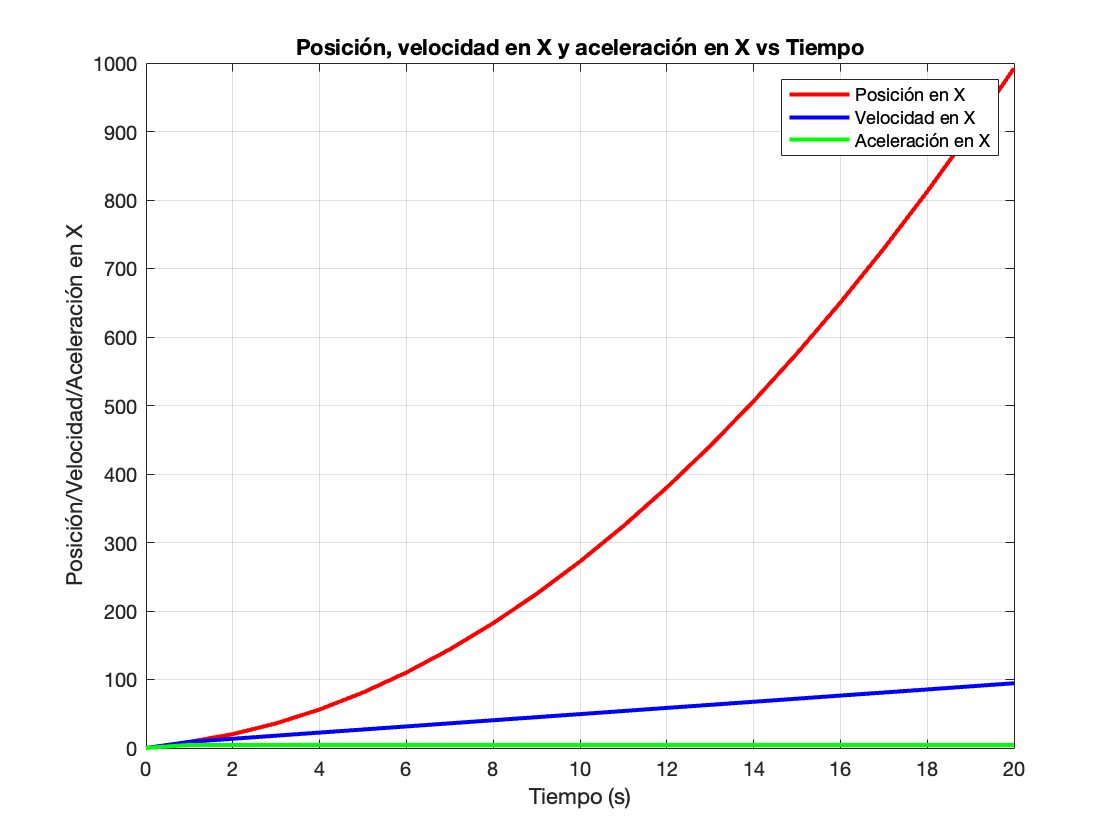
\includegraphics[height = 8cm]{2024-04-17_Grafica1_SeparacionMinerales.png}
    \caption{Gráfica para el Eje X}
    \label{fig:fig2}
\end{figure}
En la Figura \ref{fig:fig2}, observamos la posición, velocidad y aceleración en $X$ en el eje $Y$, y el tiempo en el eje $X$. De aquí, se puede corroborar los resultados esperados, 
la posición aumenta de acuerdo a una parábola, la velocidad aumenta en forma de una recta, y la aceleración se mantiene en constante durante todo el periodo de graficación. Además, se observa que la posición aumenta cada vez más 
rápido en valores positivos, correspondiente al eje $X$ positivo. Además, de que la velocidad inicia en $0$m/s y termina aproximadamente en $100$m/s. Por último, la aceleración se mantiene 
en un valor de $4.5\frac{m}{s^2}$. Éstos resultados son congruentes con el modelo matemático, y lo reflejan fielmente. \\

Continuando con el caso de prueba, se muestra la gráfica para el Eje $y$: 
\begin{figure}[H]
    \centering
    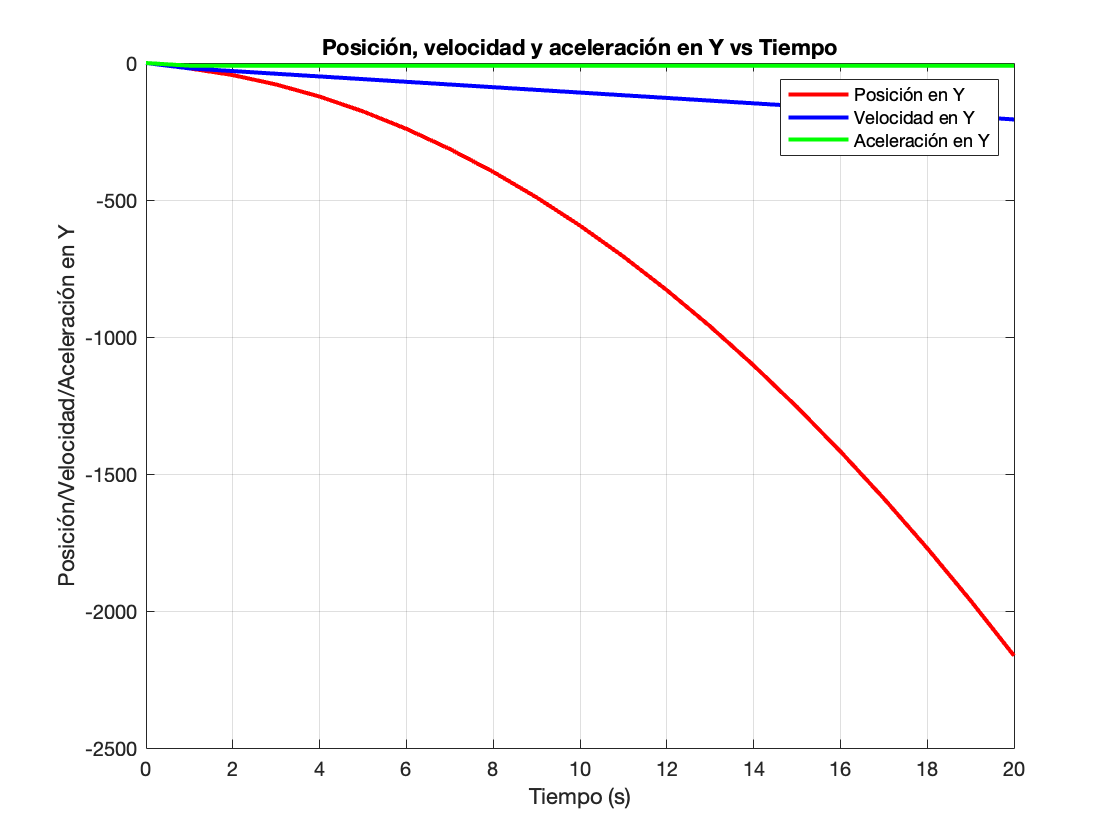
\includegraphics[height = 8cm]{2024-04-17_Grafica2_SeparacionMinerales.png}
    \caption{Gráfica para el eje y}
    \label{fig:fig3}
\end{figure} En el caso de la Figura \ref{fig:fig3}, encontramos que la aceleración en Y se mantiene constante en $9.81\frac{m}{s^2}$, mientras que la velocidad es negativa y disminuye conforme a una recta, congruente 
con el modelo matemático. Por último, la posición nos indica que se mueve en el eje $Y$ negativo, lo que indica que efectivamente se mueve hacia adentro de la cámara, 
y junto con el movimiento en el eje $X$, se mueve hacia uno de los polos. Ésto lo vemos porque la línea de posición en $Y$ decrece cade vez más lento. 

\subsection*{Relevancia Industrial}
Un simulador como el presentado en éste reporte tiene mucha importancia en la industria. Principalmente en las plantas de procesamiento, se puede usar 
para optimizar procesos de separación mineral, así maximizando la recuperación de minerales valiosos. Además, permiten predecir el rendimiento de la separación de minerales bajo 
diferentes condiciones, lo que ayuda a mejorar la calidad de los procesos. Por último, puede ayudar a las empresas en éste sector a 
desarrollar estrategias para reducir las pérdidas en base al comportamiento de éstas partículas en el simulador. 
\end{document}